\subsection{A decoupled per-group ensemble}
\label{sec:yolo_ensemble}

The two experiments above show that a single monolithic detector is dominated by whichever class is most frequent. The natural next step is to decouple the problem: instead of one seven-class model, a small ensemble of specialised detectors, each trained only on morphologically similar classes so that high-frequency features cannot overwhelm the gradient signal of rare ones.

Classes are grouped by geometry: a two-dimensional (areal) group $f_1$ --- impact craters, pit skylights, irregular mare patches, Apollo sites --- and a one-dimensional (curvilinear) group $f_2$ --- wrinkle ridges, lobate scarps, candidate rilles. Within each group, the dominant class receives a dedicated single-class detector and the remaining classes share a second detector, yielding four YOLOv8n models: (1) craters only, (2) pit/mare-patch/Apollo, (3) wrinkle ridges only, (4) scarp/rille. Each model is trained on the subset of tiles containing boxes of its classes, with the box-extraction and size-gate procedure described above (Fig.~\ref{fig:yolo_ensemble_cm} shows the validation confusion matrices of the two multi-class members).

\begin{figure}[htbp!]
\centering
\begin{subfigure}[b]{0.48\columnwidth}
    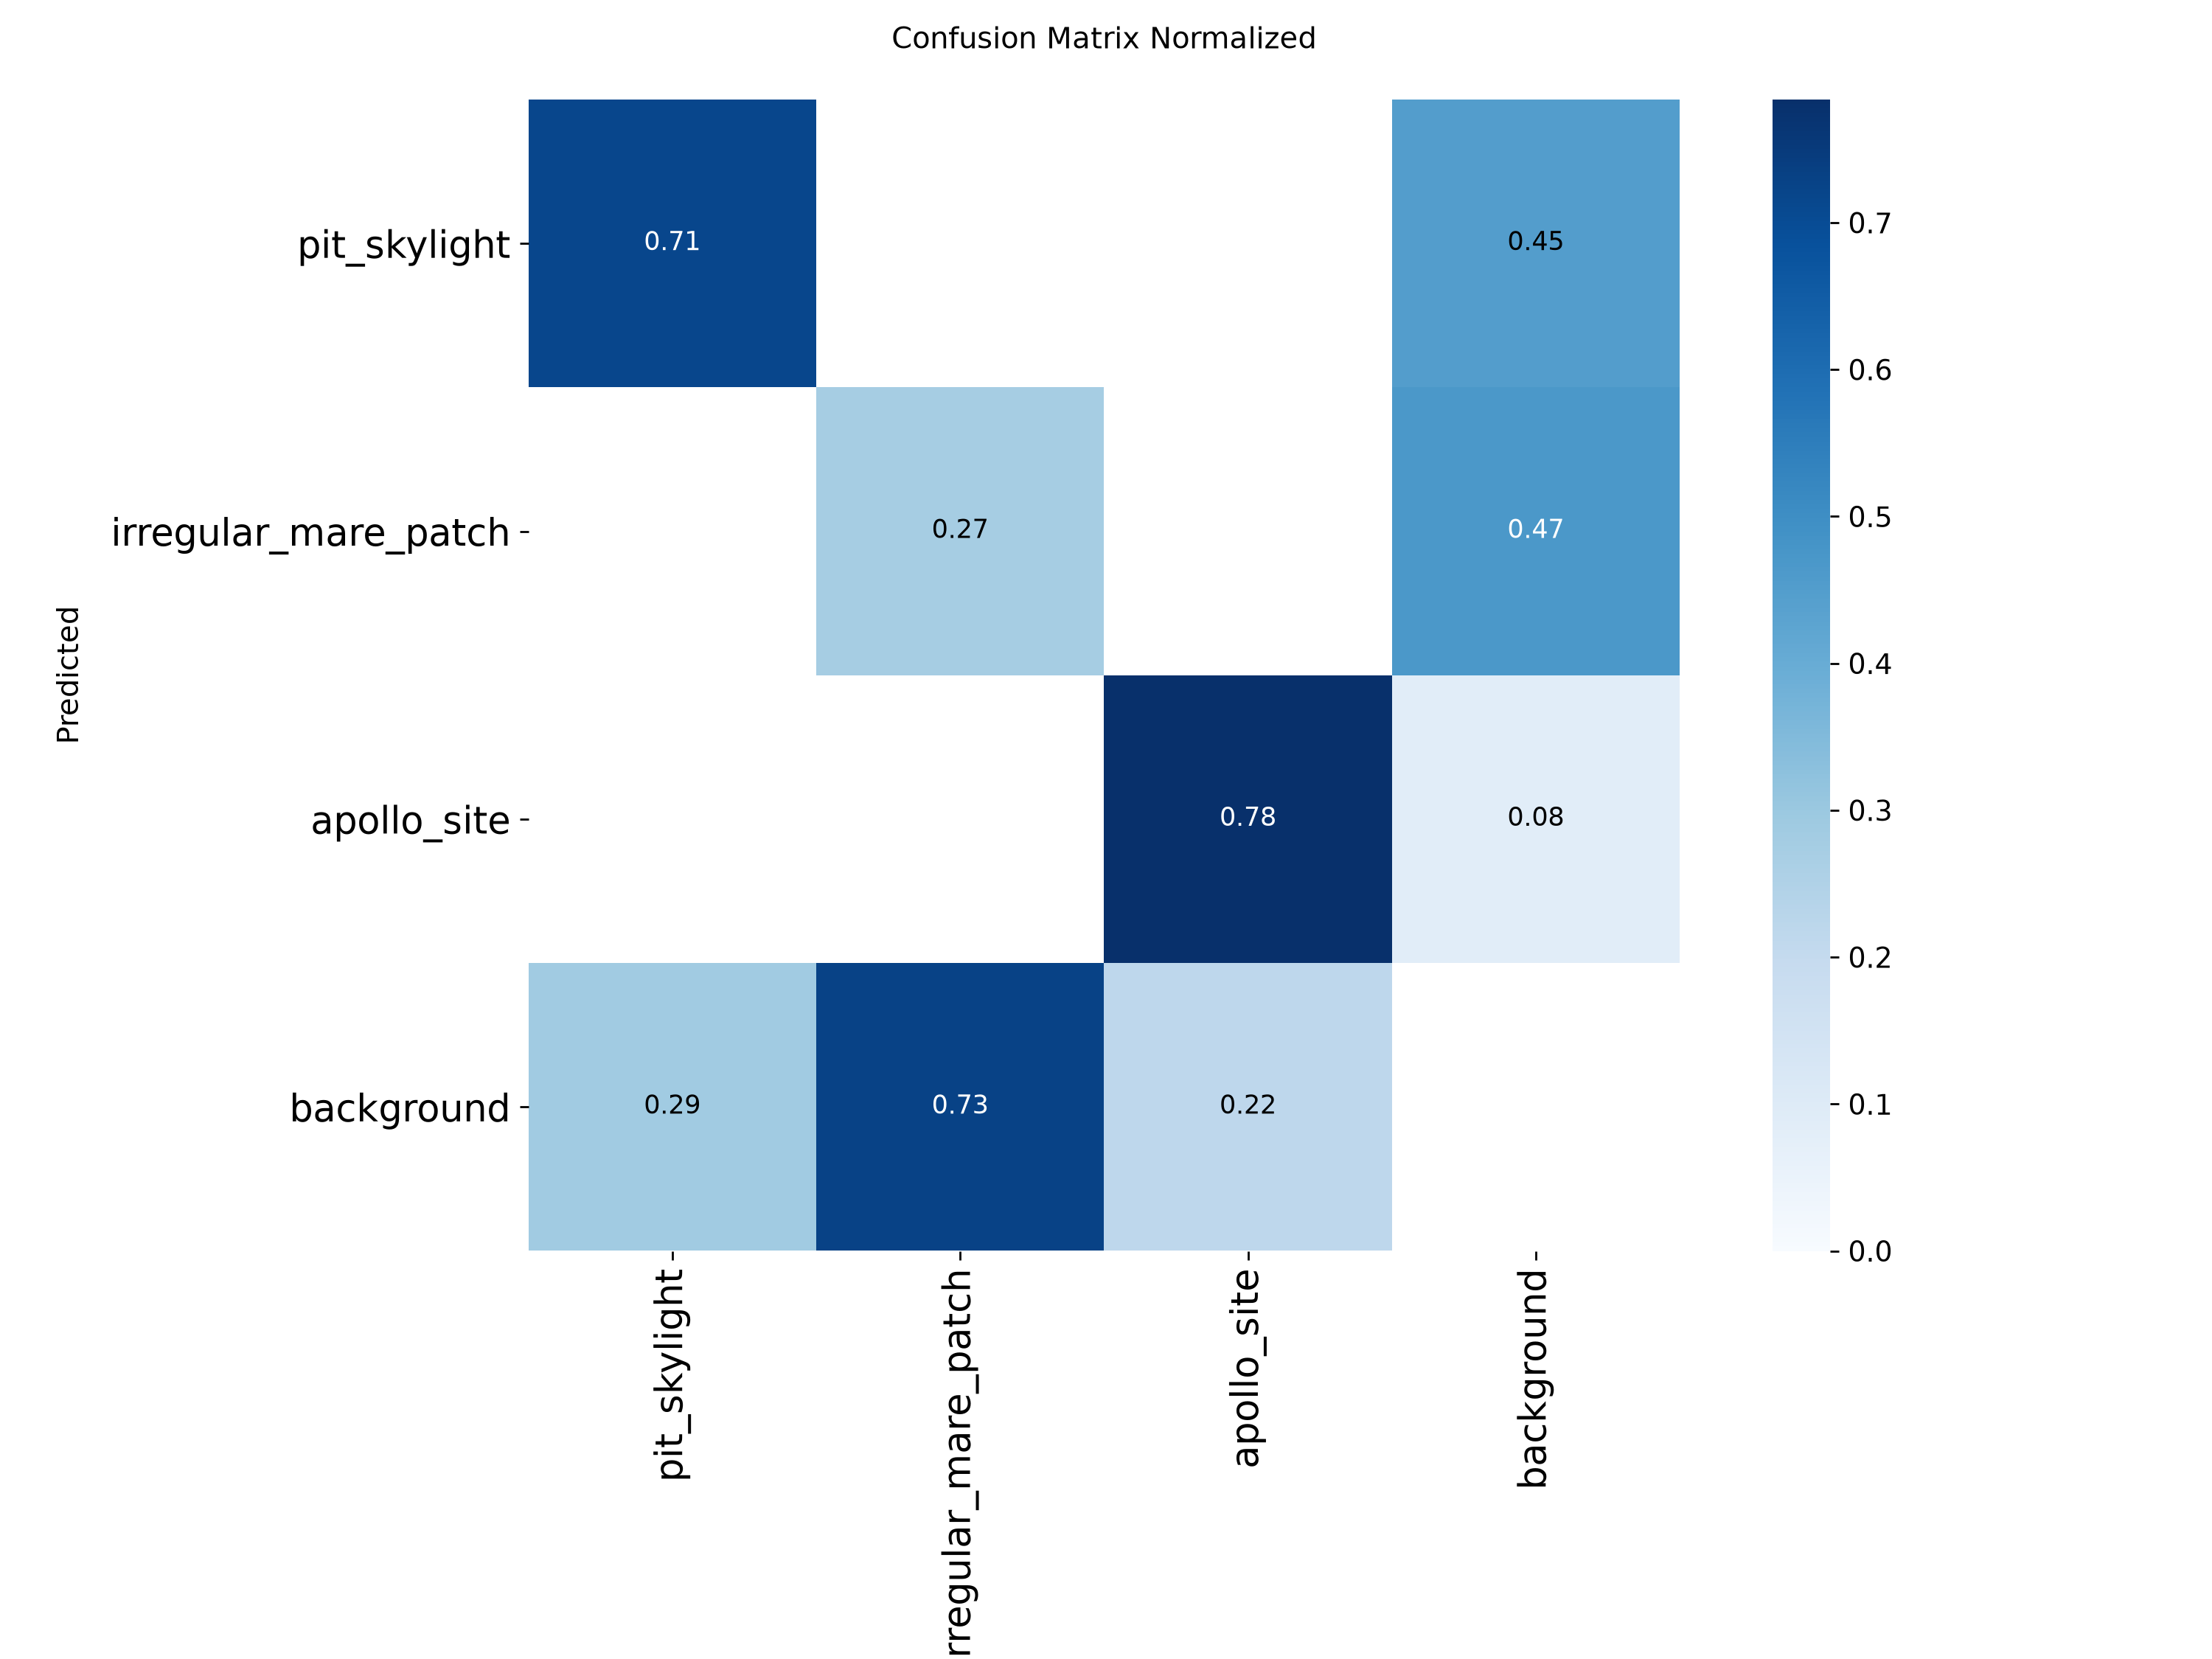
\includegraphics[width=\textwidth]{figures/YOLO/YOLO_f1.2_matrix.png}
    \caption{$f_1$ group model.}
\end{subfigure}
\hfill
\begin{subfigure}[b]{0.48\columnwidth}
    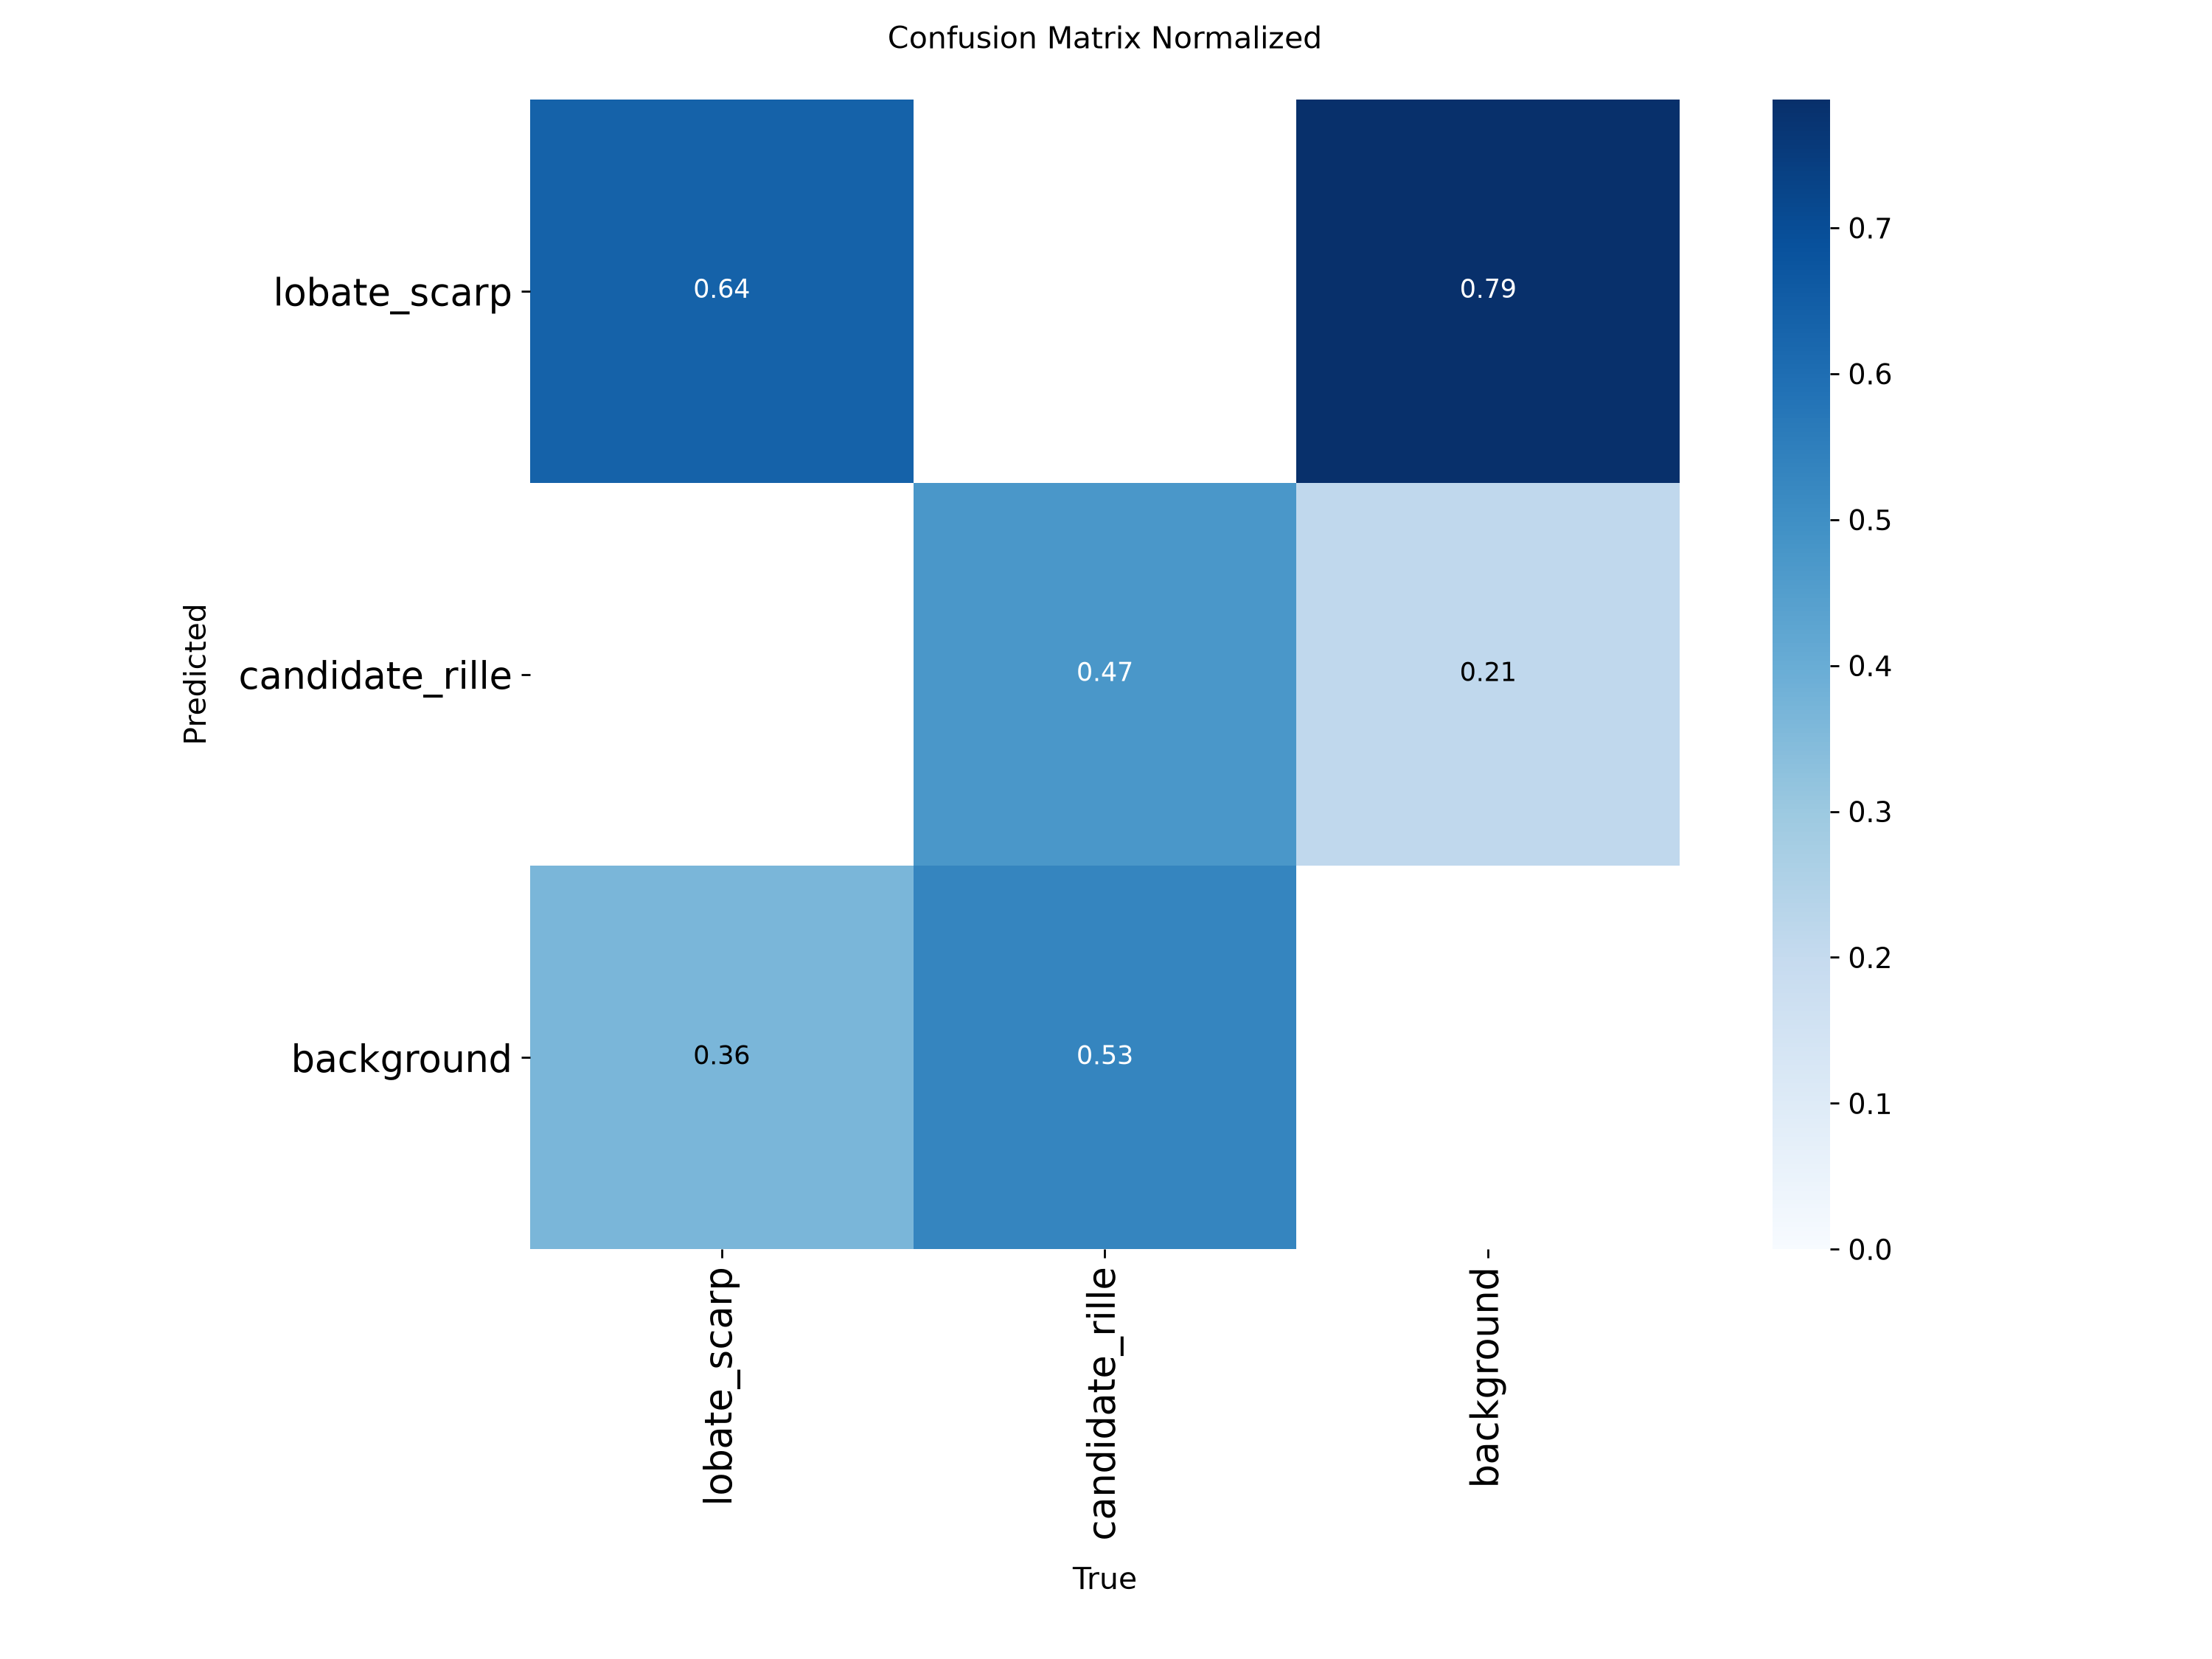
\includegraphics[width=\textwidth]{figures/YOLO/YOLO_f2.2_matrix.png}
    \caption{$f_2$ group model.}
\end{subfigure}
\caption{Normalised validation confusion matrices of the two multi-class ensemble members (random-split protocol). Diagonal dominance shows that within a morphological group the rare classes are separable once the dominant class is removed; confusion with background remains the main error mode.}
\label{fig:yolo_ensemble_cm}
\end{figure}

On the random-split protocol used during development, the training-run validation scores of the two single-class members reached mAP50 $\approx 0.9$, while the rare multi-class members remained much lower ($\approx$0.50 for the $f_1$ group and $\approx$0.25 for the $f_2$ group). These development scores are not comparable to the numbers of Sect.~\ref{sec:comparison}: they are measured on a random split over 50\%-overlapping tiles, on datasets restricted to feature-bearing tiles, and at a different training budget. Sect.~\ref{sec:split_study} disentangles exactly this: it retrains the two single-class detectors of the ensemble --- the crater and the wrinkle-ridge model --- under the random and the spatial protocol at matched budget, making the ensemble's headline members directly commensurable with the rest of the paper.
